% This is samplepaper.tex, a sample chapter demonstrating the
% LLNCS macro package for Springer Computer Science proceedings;
% Version 2.20 of 2017/10/04
%
\RequirePackage{amsmath} %% when preloaded the llncs can redefine
%                        %% things without problems.
%
\documentclass[runningheads]{llncs}
%
\usepackage{amsmath,amssymb,amsthm}
\usepackage{phonetic}
\usepackage{fancyhdr}
\usepackage[pass]{geometry}
\usepackage{fontspec}
\usepackage{url}
\usepackage{booktabs}
\usepackage[table,xcdraw]{xcolor}

\usepackage{xunicode}
\usepackage{xltxtra}
%\usepackage{xgreek}
\setmainfont[Mapping=TeX-text]{Times New Roman}
\usepackage{hyperref}
\hypersetup{
    colorlinks=true,       % false: boxed links; true: colored links
    linkcolor=blue,          % color of internal links (change box color with linkbordercolor)
    citecolor=red,        % color of links to bibliography
    filecolor=magenta,      % color of file links
    urlcolor=cyan           % color of external links
}
\usepackage[dvipsnames]{xcolor}
\usepackage[Glenn]{fncychap}
\ChNameVar{\bfseries\Large}
\usepackage{tabularx}
\usepackage[normalem]{ulem}

%% myPackages (Extra)
\usepackage{enumitem}

\renewcommand{\maketitle}{
  \begin{titlepage}
    \newgeometry{left=4cm, top=2.3cm, bottom=2.3cm}

    \hbox{
      \mbox{ \hspace{-1.3cm} }
      \vrule depth 0.98 \textheight
      \mbox{ \hspace{1cm} }

        \vtop{
          \vspace{2cm}

          \begin{flushleft}
            \huge{\bf Thesis Title\\}
            \vskip3cm
            \Large  Author's name\\
            Author's Registration Number\\
            \vskip3cm

            \begin{minipage}{7.5cm}
              \begin{flushleft}
                \normalsize {\it {\bf Examination committee:}\\
                Professor's name, Department or School, Institution.\\
                Professor's name, Department or School, Institution.\\
                Professor's name, Department or School, Institution.}
              \end{flushleft}
            \end{minipage}

            \hskip0.5cm
            \begin{minipage}{6cm}
              \begin{flushleft}
                \normalsize {\it {\bf Supervisor:}\\
                Supervisor's name, Rank, \\ Department or School,\\
                Institution.\\
                }
              \end{flushleft}
            \end{minipage}

          \end{flushleft}

          \vskip6cm
          \hskip4.5cm
          \begin{minipage}{5cm}
            \begin{center}
              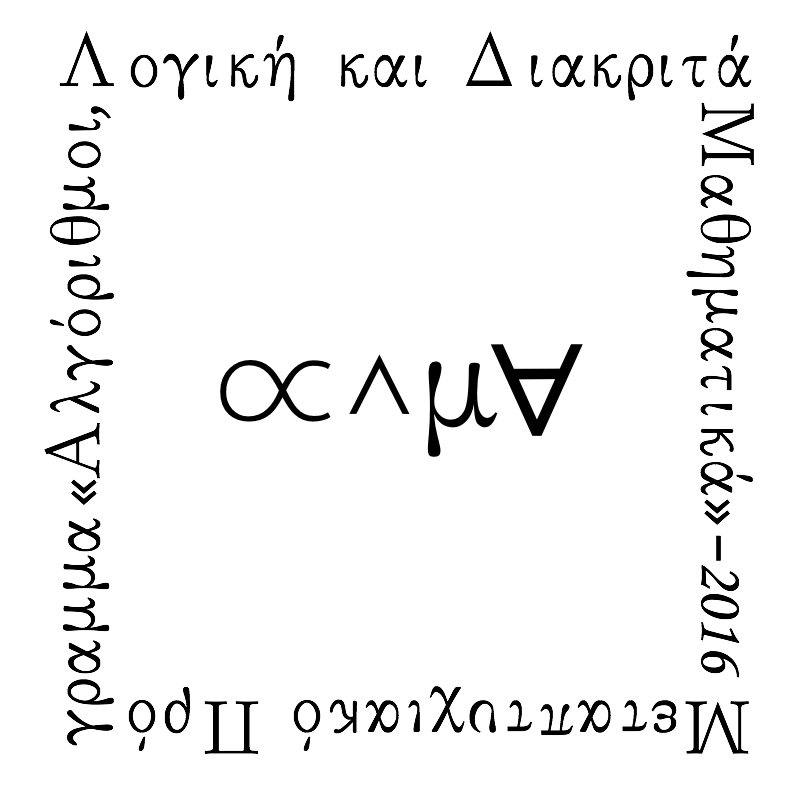
\includegraphics[width=0.8\textwidth]{alma.png}
            \end{center}
          \end{minipage}
        }
    }

 \end{titlepage}
 }

 %%%%%%%%%%%%%%%%%%%%%%%%%%%%%%%%%%%%%%%%%%%%%%%%%%%%%%%%%%%%%%%%%%%%%%%%
 %%%%%%%%%%%%%%%%%%%%%%%%%%%%%%%%%%%%%%%%%%%%%%%%%%%%%%%%%%%%%%%%%%%%%%%%

\theoremstyle{definition}
\newtheorem{ex}{}[section]
\newtheorem{definition}{Definition}[chapter]
\newtheorem{theorem}[definition]{Theorem}
\newtheorem{lemma}[definition]{Lemma}
\newtheorem{corollary}[definition]{Corollary}
\theoremstyle{remark}
\newtheorem{example}[definition]{Example}
\newtheorem{claim}[definition]{Claim}

%%%%%%%%%%%%%%%%%%%%%%%%%%%%%%%%%%%%%%%%%%%%%%%%%%%%%%%%%%%%%%%%%%%%%%%%%
%%%%%%%%%%%%%%%%%%%%%%%%%%%%%%%%%%%%%%%%%%%%%%%%%%%%%%%%%%%%%%%%%%%%%%%%%

\fancyhead[LO]{\slshape \leftmark}
\fancyhead[RE]{\slshape \rightmark}
\fancyhead[LE]{}
\fancyhead[RO]{}
\fancyfoot[LO,RE]{
\tiny{\it}}

%
\begin{document}
%
\title{Contribution Title\thanks{Supported by organization x.}}
%
%\titlerunning{Abbreviated paper title}
% If the paper title is too long for the running head, you can set
% an abbreviated paper title here
%
\author{First Author\inst{1}\orcidID{0000-1111-2222-3333} \and
Second Author\inst{2,3}\orcidID{1111-2222-3333-4444} \and
Third Author\inst{3}\orcidID{2222--3333-4444-5555}}
%
\authorrunning{F. Author et al.}
% First names are abbreviated in the running head.
% If there are more than two authors, 'et al.' is used.
%
\institute{Princeton University, Princeton NJ 08544, USA \and
Springer Heidelberg, Tiergartenstr. 17, 69121 Heidelberg, Germany
\email{lncs@springer.com}\\
\url{http://www.springer.com/gp/computer-science/lncs} \and
ABC Institute, Rupert-Karls-University Heidelberg, Heidelberg, Germany\\
\email{\{abc,lncs\}@uni-heidelberg.de}}

\maketitle              % typeset the header of the contribution
\begin{abstract}
The abstract should briefly summarize the contents of the paper in
15--250 words.

\keywords{First keyword  \and Second keyword \and Another keyword.}
\end{abstract}

%
\newpage
\pagenumbering{Roman}
\setcounter{page}{1}
\thispagestyle{headings}
\pdfbookmark{\contentsname}{toc}
\tableofcontents
\newpage
\phantomsection
\cleardoublepage

%
%
\pagenumbering{arabic}
\setcounter{page}{1}
%
%
\setcounter{chapter}{-1}
\chapter{Introduction}
%
\section{Overview}
%
%
%
\section{Thesis structure}
what is wrong?~\cite{Daemen99aesproposal:}

\chapter*{Preliminaries}
\addcontentsline{toc}{chapter}{Preliminaries}
%
\setcounter{section}{0}
\section{Overview}
%
\section{Hash function}
%
In this section, we will define the syntax and the security model of the cryptographic hash function, as introduced in \cite{Katz:2007:IMC:1206501}. We will slightly change their definition, because we assume no key as input to the hash function. In our case, the only input is a message.
%
\begin{definition}{(Hash function - syntax)} \textnormal{\cite{Katz:2007:IMC:1206501}}
A \textbf{hash function} is a probabilistic polynomial-time algorithm $H$
fulfilling the following:
\begin{itemize}
  \item[$\bullet$] There exists a polynomial $l$ such that $H$ is (deterministic) polynomial-time
  algorithm that takes as input any string $x \in { \{ 0,1 \}}^*$, and outputs
  a string $H(x) \in { \{ 0,1 \}}^{l(n)}$.
\end{itemize}
If for every $n$, $H$ is defined only over inputs of length $l'(n)$ and $l'(n) > l(n)$, then
we say that $H$ is a \textbf{fixed-length hash function} with length parameter $l'$. The output of a hash function is called digest.
\end{definition}

Notice that in the fixed-length case we require that $l'$ be greater than $l$. This ensures that the
function is a hash function in the classic sense in that it \textit{compresses} the input. We remark
that in the general case we have no requirement on $l$ because the function takes for input all (finite) binary strings. Thus, by definition, it also compresses.

We will now define security for this model. We begin by defining a game for a hash function $H$, an adversary $\mathcal{A}$ and a security parameter $n$:
\\

\textbf{The collision-finding game ${Hash-coll}_{\mathcal{A},H}(n)$:} \cite{Katz:2007:IMC:1206501}
\begin{enumerate}
  \item The adversary $\mathcal{A}$ outputs a pair $x$ and $x'$. \\
  Formally, $(x,x') \leftarrow \mathcal{A}(s)$.
  \item The output of the experiment is $1$ if and only if $x \neq x'$ and $H(x) = H(x')$. In such a case we say that $\mathcal{A}$ has found a collision.
\end{enumerate}
%
The definition of collision resistance for hash functions states that no efficient adversary can find a collision except with negligible probability.
%
\begin{definition} \textnormal{\cite{Katz:2007:IMC:1206501}}
  A hash function $H$ is \textbf{collision resistant} if for all probabilistic polynomial-time adversaries $\mathcal{A}$ there exists a negligible function $\textbf{negl}$ such that

\begin{equation}\label{eqn:collision}
  Pr[{Hash-coll}_{\mathcal{A},H}(n) = 1] \leq \textbf{negl} \: (n)
\end{equation}
\end{definition}
%
\section{Memory-Hard Functions}
In this section we will define the notion of the memory-hard function in the Parallel Random Oracle Model (pROM) of \cite{Alwen:2015:HPC:2746539.2746622}, as introduced in \cite{cryptoeprint:2016:875}. First, we will define the model along with the associated complexity notions.

\paragraph{The parallel Random Oracle Model.} We consider an algorithm $\mathcal{A}$ executing in the pROM of computation \cite{Alwen:2015:HPC:2746539.2746622}. Let this algorithm be repeated an arbitrary amount of times. After each invocation we make states. At invocation $i \in \{ 1,2, \dots \}$ algorithm $\mathcal{A}$ keeps the state $\sigma_{i-1}$ it produced. Next $\mathcal{A}$ can make calls $\textbf{q}_i = (q_{1,i}, q_{2,i}, \dots)$
to the \textit{fixed input length random oracle $H$} (ideal compression function). After it receives the digest of $H$, is allowed to perform arbitrary computation before producing its output (the next state $\sigma_i$). The state $\sigma_0$ contains the input to the computation and no other state is kept by $\mathcal{A}$. Now, we need some complexity notions to be defined.

The cumulative memory complexity (CMC) is defined to be
\begin{equation}
    cmc(\mathcal{A}) = \underset{H}{\mathbb{E}} \Bigg{[} \underset{x,r}{\max} \sum_{i} \lvert \sigma_i \rvert \Bigg{]}
\end{equation}
where $\lvert \sigma \rvert$ is the bit-length of state $\sigma$, the expectation is taken over the choice of $H$ and $max_{x,r}$ denotes the maximum over all inputs and coins of $\mathcal{A}$.

Moreover, the \textit{time complexity} (TC), $time(\mathcal{A})$ is the maximum running time of $\mathcal{A}$ in any execution. Similarly, the \textit{space complexity} (SC) is the largest state it ever outputs in any execution.

\paragraph{Oracle function.} Let $f$ be a function over strings depending on the choice of $H$. We consider the scenario in which we want to compute $f$ on $m \in \mathbb{N}^{+}$ arbitrary distinct inputs.
Let $\mathbb{A}_{f,m,q}$ be the set of pROM algorithms that accomplish this, making at most $q$ queries to
$H$. Then,

\begin{enumerate}[label=(\alph*)]
  \item $f$ is an oracle function \\

  \item The \textit{amortized cumulative memory complexity} (aCMC) of $f$ is defined to be
  \begin{equation}
      cmc_{m,q}(f) = \min \Bigg{\{} \frac{cmc(\mathcal{A})}{n} : \: n \in [m], \mathcal{A} \in \mathbb{A}_{f,n,q} \Bigg{\}}.
  \end{equation}
\end{enumerate}
This definition provides a good lower-bound on the \textit{amortized time complexity} of a function \cite{Alwen:2015:HPC:2746539.2746622}.

For more detailed information about the above, we refer the reader to the appendix of \cite{cryptoeprint:2016:875}. There are some technical details there that are beyond the scope of this thesis. Now we are ready to define properly the notion of the memory-hard function.

\begin{definition}{\textbf{(Memory-Hard Function).}} \textnormal{\cite{cryptoeprint:2016:875}}
  Let $\{ f_{\sigma, \tau} \}_{\sigma, \tau \in \mathbb{N}^{+}}$ be a family of (oracle) functions and $\mathcal{N}$ be a sequential pROM algorithm which, on input $(\sigma, \tau, x)$, outputs $f_{\sigma, \tau}(x)$ in time at most $\tau \sigma$ using space at most $\sigma$. Then $F=\big{(} \{ f_{\sigma,\tau} \}, \mathcal{N} \big{)}$
  is an $(h,g,t)$-memory-hard function (for up to $m$ instances and $q$ queries) if it has memory-hardness at least $h$, memory-gap at most $g$ and throughput at least $t$ (all functions of $\sigma$ and $\tau$).

\begin{align*}
cmc_{m,q}(f_{\sigma, \tau})&\geq h(\sigma, \tau)           &  \frac{\mbox{space}(\mathcal{N})*\mbox{time}(\mathcal{N})}{cmc_{m,q}(f_{\sigma, \tau})} &\leq g(\sigma, \tau)             &  \frac{\mbox{space}(\mathcal{N})}{\mbox{time}(\mathcal{N})} &\geq t(\sigma, \tau)\\
\end{align*}
%
\end{definition}
%
\section{Pseudorandom Functions}
In cryptography, a pseudorandom function family, abbreviated $PRF$, is a collection of efficiently-computable functions which emulate a random oracle in the following way: no efficient algorithm can distinguish (with significant advantage) between a function chosen randomly from the PRF family and a random oracle (a function whose outputs are fixed completely at random). With that in mind,
we must first recall the definition of oracle indistinguishability and then proceed to define a pseudorandom function.

\begin{definition}{(Oracle Indistinguishability).} \textnormal{\cite{ACI}}
  Let $\{ O_n \}_{n \in \mathbb{N}}$ and $\{ O'_{n} \}_{n}$ be ensembles where $O_n, O'_n$ are probability
  distributions over functions $f: \{ 0,1 \}^{l_1(n)} \rightarrow \{ 0,1 \}^{l_2(n)}$ for some polynomials $l_1(\cdot)$, $l_2(\cdot)$. We say that $\{ O_{n} \}_{n}$ and $\{ O'_{n} \}_{n}$ are \textbf{computationally indistinguishable} (denoted by $\{ O'_{n} \}_{n} \approx \{ O'_n \}_{n \in \mathbb{N}}$
  ) if for all non-uniform p.p.t. oracles machines $D$, there exists a negligible function $\epsilon(\cdot)$ such that $\forall n \in \mathbb{N}$
  \begin{equation}{\label{oracle}}
    \Bigg{\lvert} \: Pr \big{[} F \leftarrow O_n : D^{F(\cdot)}(1^n)=1 \big{]} - Pr \big{[} F \leftarrow O'_n : D^{F(\cdot)}(1^n)=1 \big{]} \: \Bigg{\rvert} < \epsilon(n).
  \end{equation}
\end{definition}

\begin{definition}{(Pseudo-random Function).} \textnormal{\cite{ACI}}
  A family of functions $\big{\{} f_s: \{ 0,1 \}^{\lvert s \rvert} \rightarrow \{ 0,1 \}^{\lvert s \rvert} \big{\}}_{s \in \{ 0,1 \}^{*}}$ is \textbf{pseudo-random} if
  \begin{itemize}
    \item[$\bullet$] (Easy to compute): $f_s(x)$ can be computed by a p.p.t. algorithm that is given input $s$ and $x$
    \item[$\bullet$] (Pseudorandom): $\big{\{} s \leftarrow \{ 0,1 \}^n: f_s \big{\}}_n \approx \big{\{} F \leftarrow RF_n: F \big{\}}_n$.
  \end{itemize}
\end{definition}
Notice that if someone knows $s$ then it is easy to distinguish $f_s$ from a random function. In order to consider this function indistinguishable from a random function, one should keep seed $s$ secret.
%
%
%% Password scramblers
%
%% Pebbling game
%
%% Information about pebbling algorithms and complexity

\chapter*{Cryptocurrency Mining}
\addcontentsline{toc}{chapter}{Cryptocurrency Mining}
%
\setcounter{section}{0}
\section{Overview}
%
\section{Bitcoin}
Bitcoin~\cite{Nakamoto_bitcoin:a} is a decentralized digital currency that enables instant payments to anyone, anywhere in the world. Bitcoin uses peer-to-peer technology to operate with no central authority: transaction management and money issuance are carried out collectively by the network.

The original Bitcoin software by Satoshi Nakamoto was released under the MIT license. Most client software, derived or "from scratch", also use open source licensing.

Bitcoin is the first successful implementation of a distributed crypto-currency, described in part in 1998 by Wei Dai on the cypherpunks mailing list. Building upon the notion that money is any object, or any sort of record, accepted as payment for goods and services and repayment of debts in a given country or socio-economic context, Bitcoin is designed around the idea of using cryptography to control the creation and transfer of money, rather than relying on central authorities.

Bitcoins have all the desirable properties of a money-like good. They are portable, durable, divisible, recognizable, fungible, scarce and difficult to counterfeit.

%
\section{Mining}
Bitcoin mining\footnote{It is misleading to think that there is an analogy between gold mining and bitcoin mining. The fact is that gold miners are rewarded for producing gold, while bitcoin miners are not rewarded for producing bitcoins; they are rewarded for their record-keeping services.} is the processing of transactions in the digital currency system, in which the records of current Bitcoin transactions, \textit{blocks}, are added to the record of past transactions, the \textit{blockchain}. Miners keep the blockchain consistent, complete, and unalterable by repeatedly grouping newly broadcast transactions into a block, which is then broadcast to the network and verified by recipient nodes.~\cite{economist} Each block contains a SHA-256 cryptographic hash of the previous block~\cite{economist}, thus linking it to the previous block and giving the blockchain its name.

To be accepted by the rest of the network, a new block must contain a proof-of-work ($PoW$). The system used is based on Adam Back's 1997 anti-spam scheme, Hashcash~\cite{Nakamoto_bitcoin:a}.
The $PoW$ requires miners to find a number called a nonce, such that when the block content is hashed along with the nonce, the result is numerically smaller than the network's difficulty target~\cite{Nakamoto_bitcoin:a}. This proof is easy for any node in the network to verify, but extremely time-consuming to generate, as for a secure cryptographic hash, miners must try many different nonce values before meeting the difficulty target.

The primary purpose of mining is to set the history of transactions in a way that is computationally impractical to modify by any one entity. By downloading and verifying the blockchain, bitcoin nodes are able to reach consensus about the ordering of events in bitcoin.~\cite{wiki}

Every 2,016 blocks (approximately 14 days at roughly 10 min per block), the difficulty target is adjusted based on the network's recent performance, with the aim of keeping the average time between new blocks at ten minutes. In this way the system automatically adapts to the total amount of mining power on the network. Between 1 March 2014 and 1 March 2015, the average number of nonces miners had to try before creating a new block increased from 16.4 quintillion to 200.5 quintillion.\cite{difficulty_history}

The proof-of-work system, alongside the chaining of blocks, makes modifications of the blockchain extremely hard, as an attacker must modify all subsequent blocks in order for the modifications of one block to be accepted. As new blocks are mined all the time, the difficulty of modifying a block increases as time passes and the number of subsequent blocks (also called confirmations of the given block) increases.~\cite{economist}

Mining is also the mechanism used to introduce Bitcoins into the system: Miners are paid any transaction fees as well as a "subsidy" of newly created coins. This both serves the purpose of disseminating new coins in a decentralized manner as well as motivating people to provide security for the system.~\cite{wiki}

Originally, Bitcoin mining was conducted on the \textit{CPUs} of individual computers, with more cores and greater speed resulting in more profitability. After that, the system became dominated by multi-graphics card systems, then field-programmable gate arrays (\textit{FPGAs}) and finally application-specific integrated circuits (\textit{ASICs}), in the attempt to find more hashes per hour with less electrical power usage.

Due to this constant escalation, it has become hard for prospective new miners to start. This adjustable difficulty is an intentional mechanism created to prevent inflation. To get around that problem, individuals often work in mining pools.

Bitcoin generally started with individuals and small organizations mining. At that time, start-up could be enabled by a single high-end gaming system. Now, however, larger mining organizations might spend tens of thousands on one high-performance, specialized application-specific integrated circuit.

That creates a problem. In a system, which from its creation, it is supposed to distribute power among users, there has been a great power concentration in the hands of big companies, like Bitfury or 21, that develop ASICs to mine bitcoin. Because of the extreme cost of ASICs and extreme hashrate, someone who uses a multi-graphics card system or a $CPU$ is out of competition. As a result of this, independent miners have largely dried up.

%
\section{Egalitarian Mining}
Let's consider several contexts where an adversary has an upper hand over the defender by using special hardware in an attack. These include password processing, hard-drive protection, cryptocurrency mining, resourse sharing, code obfuscation, etc. Memory-hard computing is a generic paradigm, which can protect the defender against attacks in the aforementioned contexts. Every task is amalgamated with a certain procedure requiring intensive access to $RAM$ both in terms of size and bandwidth, so that transferring the computation to $GPU$, $FPGA$, and even $ASIC$ brings little or no cost reduction. Cryptographic schemes that run in this framework become \emph{egalitarian} in the sense that both users and attackers are equal in the price-performance ratio conditions. When the cryptographic scheme is a hash fuction used for cryptocurrency mining, then we refer to this notion as \emph{egalitarian mining}.

But let's step back a little and think about the need for such a notion. Do we actually need it? Is egalitarian mining a way to destroy competition? Is it unfair? Shouldn't a miner be rewarded for the extra money he invested?

Many questions like the above have been asked and usually the answer is not descriptive enough of what really memory-hardness introduces to the world. We will try here to demonstrate exactly what it means for a coin to offer egalitarian mining.

\emph{Egalitarian mining does not destroy competition.} The miner who invests more in hardware, is rewarded more. Each individual miner is rewarded according to the computation power he offers to the coin. The real difference is that it is really easy for people to start mining with a single high-end gaming system. Hobbists, who want to support the community are welcome to mine. In bitcoin system, this option is not available. In order to support the coin by mining, you have to invest a lot of money on ASICs to be competitive. That means, that in general, the mining for support or for fun, is dead.

This is hurtful for a system, which by design is supposed to bring decentralization in the financial market. That is because without hobbists we are actually left with big companies handling almost all of the mining. Companies will comply with regulations that the government of each country enforces and cannot be expected to react and inspire movements. Since countries can and they have, historically, collaborated against threats, a union of countries who can enforce regulations to companies, that control more than 51\% of the hashing power, can bring a coin to its knees, if seen as a threat. That scenario, does not fit in most definitions of security.

One of the reasons that coins have a bootstrapping period is because they need a big society to distribute mining, in order to guarantee security. When the total hashing power is a few high-end gaming systems, aquaring 51\% of the hashing power is unfeasible. As the support expands, the security is satisfied for all practical purposes. But when mining is dominated by companies, then a totally trustless system gaves birth to a trusted party. That's against the motivation of the inception of a cryptocoin and it raises questions like "\emph{Why should I trust the mining companies and support this cryptocoin? Do I trust my bank more? After all, my bank is just another company...}"

To sum up, for reasons of security and decentralization, it is healthy for some coin's mining power to be distributed among users. Memory-hardness sustains the competition, but it makes it less harsh and keeps the door open for hobbists to support the coin. It is extremely difficult for the corporate mining to aquire tremendous power for two reasons, and that is needed in a trustless system that wants to stay trustless. The reasons are: a) it is not that lucrative for companies. If someone makes a big investment, he will get big rewards, but not insanely huge rewards leaving every hobbist out of the mining society. b) Even if a lot of companies decide to participate, it is extremely difficult for them to aquire a combined 51\% of the total hash power without destroying the "support mining" or "fun mining".

Memory-hardness defends a system against this prospect and thus strengthens the notion of coin's security. Furthermore, no matter how much someone trusts the corporations involved, security is a binary state. A system cannot be secure against attackers and insecure against other parties. It is either secure or insecure. And if the prospect of an attack exists, then security collapses.
%
\section{Monero}
Monero (XMR) is a decentralised open-source cryptocurrency forked from Bytecoin in April 2014. The coin's fundamental feature is privacy - it aims to be a digital medium of exchange with untraceable payments, unlinkable transactions and resistance to blockchain analysis. The exact person behind a Monero transaction is not known; this results in considerable increase of privacy compared to Bitcoin and its forks.~\cite{monerodef}

Monero is actively encouraged to those seeking financial privacy, since payments and account balances remain entirely hidden, which is not the standard for most cryptocurrencies.\\

\noindent Monero is:~\cite{monero}
\begin{description}
  \item [Untraceable] Monero uses a digital signature scheme called "ring signatures", which shuffles users' public keys in order to eliminate the possibility to identify a particular user.
  \item [Unlinkable] Monero employs a specific protocol which generates multiple unique one-time addresses that can only be linked by the payment receiver and are unfeasable to be revealed through blockhain analysis.
  \item [Secure] Monero is cryptographically secured. Moreover, the design of the algorithm used, consists in tremendous computational and electric capibilities that an adversary would need to even try to steal funds.
  \item [Private] Privacy is basically provided with the idea of anonymous transactions without any obligations to cooperate with third parties.
  \item [Analysis Resistant] Monero's blockhain analysis resistantce results from unlinkability, which was achieved by using a modified version of the Diffie-Hellman exchange protocol that generates multiple one-time public addresses that can only be simply gathered by the message receiver, but hardly analyzed by confused foreigners inside the block explorer.
\end{description}
%
Monero uses a Proof of Work mechanism to issue new coins and
incentivize miners to secure the network and validate transactions.
One key part, for Monero to offer the above, is a proof-of-work algorithm called CryptoNight, developed by the CryptoNote
project~\cite{citeulike:14139412}. On top of typical security attributes, this algorithm is also suspected to be memory-hard. The aim of this work is to study the memory-hardness property of this algorithm.
%
%% Cryptonight

%%%%%%%%%%%%%%%%%%%%%%%%%%%%%%%%%%%%%%%%%%%%%%%%%%%%%%
% For this chapter I need to build the figures.
% NOT done yet.
% Also need to be checked, but this will happen after
% the figure insertion.
%%%%%%%%%%%%%%%%%%%%%%%%%%%%%%%%%%%%%%%%%%%%%%%%%%%%%%

\chapter*{Cryptonight Analysis}
\addcontentsline{toc}{chapter}{Cryptonight Analysis}
%
%
\setcounter{section}{0}
\section{Description}
In this section we will describe in detail the proposed implementation of the CryptoNight hash function. This function is used in the Monero project in order to achieve \emph{egalitarian mining}. It is easy to understand why we characterize this implementation as \emph{proposed}, since each miner is free to use any implementation he/she can think of, as long as it produces the right result.

In order to prove that a function is \emph{memory-hard} we need to show that no implementation exists, that can produce the same result using less memory without a significant time cost. In other words, using an implementation which needs less memory is not something that can give advantage to some miner because the time factor will make the procedure equally or more "expensive", even if the miner uses parallel computation techniques.

\noindent Reproduced from CryptoNote~\cite{cryptonight}:
\begin{verbatim}
  CryptoNight is a memory-hard hash function. It is designed to be
  inefficiently computable on GPU, FPGA and ASIC architectures.
\end{verbatim}
In the proposed implementation, a scratchpad\footnote{a large area of memory used to store intermediate values during the evaluation of a memory-hard function.} is used (2MB) to ensure that the memory needed fits the size of L3 cache (per core) in modern processors. In practice, the miner should measure mining power and calculate efficiency. In Monero mining, $CPUs$ cores are only efficient if they can use the super fast 2MB cache over and over. Each core needs about 2MB for CryptoNight to stay cached. So a miner should check how much L2 cache or in rare cases also L3 cache the CPU has. Then divide by 2MB this, will be how many cores he/she can run at the same time.

There are several reasons to suspect that CryptoNight could be a memory-hard function. One of the most popular argument was that a megabyte of internal memory is an almost unacceptable size for a modern ASIC pipeline. But, hardware is evolving and eventually there was recently an effort for Monero \emph{ASIC} production.

There were some thoughts like "\emph{How did they did this? Isn't CryptoNight memory-bound?}". Well, one thing is that CryptoNight is \emph{ASIC-resistant}, not \emph{proof}. But, that was not the case. Another issue is that L3 cache supports a lot of extra functionality like being shared across cores, writing back to $RAM$, being behind two other levels of cache, etc. which all makes a lot less efficient (among other issues with the approach). But, again, that was not the case in that particular effort.

L3 latency wasn't the issue. The $ASICs$ just traded latency for bandwidth the same way $GPUs$ do. They're built on stacks of $DRAM$ not lightning fast caches. The costs of cache complexity aren't only latency but also power usage and die space. Raw speed isn't even necessarily the goal for either $CPUs$ or $GPUs$ or $ASICs$ here, it is efficiency.

But, Monero project reacted and announced upgrades bi-annually in order to keep ASIC's at bay. Upgrades are a problem, because upgrades produce bugs and vulnerabilities. Especially, when they are that frequent. On the other hand, upgrades in Monero are minor with no changes to the memory-hard part. From this experience we understand that a formal proof or even a better understanding of the memory-hardness property in practice, is vital in order to protect a cryptocurrency from centralization.

In this chapter we will just show the proposed implementation of CryptoNight without any analysis. We will demonstrate the three stages of the computation and the role for each element. A really quick overview of these stages would be something like this:

\begin{enumerate}
  \item Initialize the scratchpad in a pseudo-random manner.
  \item Read/write operations at pseudo-random addresses. (memory-hard part)
  \item Use all the computations' results to produce the output.
\end{enumerate}

\section{The three Stages}
Enough with the overview of the function and its history. Let's dive into it and see in detail its components as it is described in \cite{cryptonight}.

The input of this algorithm is a block and if the value of the Cryptonight function satisfies the target (\hyperref[eq:target]{equation}~\ref{eq:target}), it is possible that this block is the next block in the blockchain.

\begin{equation}
  \label{eq:target}
  \color{Bittersweet} \mbox{Cryptonight}
  \color{black} (
  \color{RedViolet} \mbox{block}
  \color{black} )\leq
  \color{ForestGreen} \mbox{Target}
  \color{black}
\end{equation}
So, the input of the function is a block of transactions along with the necessary fields, which are specified by the Monero protocol.

\subsection{The first Stage}
The first stage of the algorithm sets the initial value of the scratchpad. In order to prevent several attack schemes, the scratchpad must be initialized with data chosen in a way, which is indistiguishable from the uniform distribution. This is the goal.

We will describe the first Stage in several parts and discuss the role of each part and its contribution regarding the properties of function's output. Let us begin:

\noindent Prepare the tools:
% Prepare the tools
\begin{enumerate}
  \item \label{hashing} Hash the input using Keccak~\cite{keccak} ($b=1600$, $c=512$).
  \item Choose the first $32$ bytes of the final state.
  \item Interpret them as an AES-256 key.
  \item Expand them to $10$ round keys.
\end{enumerate}
% Comment on the above
Keccak is the versatile cryptographic function that is most known as SHA-3. The parameter analysis and the description of their part is beyond the scope of this thesis. The reader is refered to their work.

We will consider Keccak a collision-free hash function. The next three steps produce random keys for encryption. We consider these keys random enough in the way that they are interpreted as keys and expanded according to \cite{nla.cat-vn4183631}.

\noindent Create the scratchpad:
\begin{enumerate}
  \setcounter{enumi}{4}
  \item Allocate $2097152$ bytes ($2$MiB).
\end{enumerate}
\noindent The encryption part:
\begin{enumerate}
  \setcounter{enumi}{5}
  \item Split the bytes $64$ to $191$ into $8$ blocks of $16$ bytes each.
  \item \label{step 7} Encrypt the blocks as follows:
    \begin{verbatim}
      for i = 0..9 do:
          block = aes_round(block, round_keys[i])
    \end{verbatim}
\end{enumerate}
\begin{enumerate}
  \setcounter{enumi}{7}
  \item Fill $128$ bytes of the scratchpad with the resulting blocks.
\end{enumerate}
\noindent Repeat:
\begin{enumerate}
  \setcounter{enumi}{8}
  \item With the resulting blocks run \hyperref[step 7]{step}~\ref{step 7} again.
\end{enumerate}
%
Each time 128 bytes are written, they represent the
result of the encryption of the previously written 128 bytes. The
process is repeated until the scratchpad is fully initialized.

\subsection{The second Stage (memory-hardness)}
The second stage of the algorithm uses the initialized scratchpad and two values that are computed from the hashed input of the function. Its goal is to perform computations on the scratchpad values (all of them, with high probability) and produce a final scratchpad structure that can't be computed otherwise or in stages (without huge time complexity). The memory-hardness property is satisfied if and only if there is no other way to compute the final stage of the scratchpad, using memory less than the size of the scratchpad. That is the intuition. In detail:

\noindent \emph{(The preparation part).} The core structure of this stage is a loop. However, before illustrating the computations that take place inside the loop, there are some computations needed for preparation and two technical clarifications.

\begin{enumerate}
  \item \label{memh: step 1} Compute the values of $a$ and $b$.
\end{enumerate}
Elements $a$ and $b$ are the two values which, along with the scratchpad, are given as input to the loop. More specifically, the first $64$ bytes of the hashed input (the Keccak state) are split in two parts ($32$ bytes each part) and $XOR$ed, and the resulting $32$ bytes are used to initialize variables $a$ and $b$, $16$ bytes each.

\noindent \emph{(Clarification 1).} The reader may notice in figure ... that the function uses a 16-byte value as an address in the scratchpad. Actually, the value is interpreted as a little-endian integer. The $21$ low-order bits are used as a byte index. To ensure the 16-byte alignment, the four low-order bits of the index are cleared. This alignment is essential, as the data is read from and written to the scratchpad in 16-byte blocks.

\noindent \emph{(Clarification 2).} The main loop is iterated $524,288 = 2^{19}$ times. Every time, two blocks of the scratchpad are written, so with high probability, the whole scratchpad will be overwritten. In every iteration, along with the two blocks of the scratchpad, values $a'$ and $b'$ are computed, which are used as input to the next iteration.

Now we are ready to describe the inner computations of the loop. We will divide this stage into parts, as it will help us later in the analysis. The number of parts are determined, based on some intermediate values. Here, we note that the intermediate values are not memory requirements, as we can implement the computations with only $32$ bytes of memory (for $a$ and $b$) plus the memory needed for the scratchpad. But during theoretical analysis and understanding of the function's computations, these intermediate values seem natural stops of the train of thought. So, after the \hyperref[memh: step 1]{step}~\ref{memh: step 1}:

\begin{enumerate}
  \setcounter{enumi}{1}
  \item \label{memh: step 2} Interpret the value of $a$ as a scratchpad address.
  \item \label{memh: step 3} Read from this address.
  \item Evaluate the AES function with data from \hyperref[memh: step 3]{step}~\ref{memh: step 3} and key the value of $a$.
\end{enumerate}
Let's call this intermediate value $c$. And let's add a final step to this part:
\begin{enumerate}
  \setcounter{enumi}{4}
  \item $XOR$ $c$ with $b$ and write the result to the address of \hyperref[memh: step 2]{step}~\ref{memh: step 2}.
\end{enumerate}
The value $c$ is passed as $b'$, part of the input of the next iteration. The second part involves another read from the scratchpad:

\begin{enumerate}
  \setcounter{enumi}{5}
  \item \label{memh: step 6} Interpret the value of $c$ as a scratchpad address.
  \item Read from this address. (We will refer to this intermediate value as $d$.)
  \item \label{memh: step 8} Multiply\footnote{The multiplication uses only the first 8 bytes of each argument, which are interpreted as unsigned 64-bit little-endian integers and multiplied together. The result is converted into 16 bytes, and finally the two 8-byte halves of the result are swapped~\cite{cryptonight}.} $c$, $d$ and add the value of $a$ to the result.
  \item Write the result of \hyperref[memh: step 8]{step}~\ref{memh: step 8} to the address of \hyperref[memh: step 6]{step}~\ref{memh: step 6}.
\end{enumerate}
This concludes the second part. The scratchpad is written twice per iteration. The only thing that is left to conclude the description of the second stage, is the computation of $a'$, part of the input of the next iteration. This is computed as follows:

\begin{enumerate}
  \setcounter{enumi}{9}
  \item $XOR$ $d$ with the result of \hyperref[memh: step 8]{step}~\ref{memh: step 8} to compute $a'$.
\end{enumerate}

\subsection{The third Stage}
The third stage of the algorithm uses the final state of the scratchpad to produce the output. During this stage $AES$ operation is used. At first, the function extracts $10$ key values from $32$ bytes of the hashed input of the function, similar to the \hyperref[hashing]{step}~\ref{hashing} of the first stage.

\noindent Extracting keys:
% Extract keys
\begin{enumerate}
  \item Choose the bytes $[32...63]$ of the final Keccak state.
  \item Interpret them as an AES-256 key.
  \item \label{keys} Expand them to $10$ round keys.
\end{enumerate}
After this, the function needs a starting value. It applies $XOR$ operation on bytes $[64...191]$ of the hashed input and the first $128$ bytes of the scratchpad. Let's call these values \emph{input} and \emph{scratchpad[0]}.

\begin{enumerate}
  \setcounter{enumi}{3}
  \item \label{xor} \emph{input} $\oplus$ \emph{scratchpad[0]}.
\end{enumerate}
Now, using the first key of \hyperref[keys]{step}~\ref{keys} as key to the $AES$ operation:

\begin{enumerate}
  \setcounter{enumi}{4}
  \item \label{encrypt} Encrypt the result of \hyperref[xor]{step}~\ref{xor}.
\end{enumerate}
Repeat the last two steps as follows:

\begin{itemize}
  \item Take as input the encrypted result of the last step.
  \item Take the next $128$ bytes of the scratchpad(\emph{scratchpad[1]}).
  \item Use, as $AES$ key, the next extracted key.
  \item Execute \hyperref[xor]{step}~\ref{xor} and \hyperref[encrypt]{step}~\ref{encrypt}.
\end{itemize}
until the last bytes of the scratchpad are used to the aforementioned operations. After the last bytes of the scratchpad are $XOR$ed and encrypted,

\begin{enumerate}
  \setcounter{enumi}{5}
  \item \label{modified} Use the result to replace the bytes $[64...191]$ of the hashed input.
\end{enumerate}
We we call the state of the hashed input after the above step as the \emph{modified Keccak state}. To produce the final result the function performs the next steps.

\begin{enumerate}
  \setcounter{enumi}{5}
  \item Pass the \emph{modified Keccak state} through Keccak-$f$ (the Keccak permutation~\cite{keccak}).
  \item Choose the 2 low-order bits of the first byte of the \emph{modified Keccak state}.
  \item Based on these bits choose a hash function:
  \begin{itemize}
    \item case $00$: BLAKE-256
    \item case $01$: Groestl-256
    \item case $10$: JH-256
    \item case $11$: Skein-256
  \end{itemize}
  \item \label{output} Apply the chosen function to the \emph{modified Keccak state}.
\end{enumerate}
The result of \hyperref[output]{step}~\ref{output} is the output of the CryptoNight function. For more information about these functions, the reader is refered to the respective articles~\cite{10030667226,sha3groestl,sha3W09,sha3F+08}.

\section{CryptoNight Analysis}
%% Introduce our model: AES as PRF, parametrize everything, set up the focus on the second stage.
% You will explain probabilities in the next chapter, but still, you can analyze the game perhaps?
% Definition of security ...? 
% A glimpse on what set of variables are NOT independent, or NOT DEFINITELY independent.
% Just set up your model, so you can write next chapter easily...
%% Still needs figures...

\chapter*{Problem Statement and our Remarks}
\addcontentsline{toc}{chapter}{Problem Statement and our Remarks}
%
%
\setcounter{section}{0}
\section{Proof approach}
%% Trying the proof approach
%
%% Trying the attack approach

\chapter{Future Work}
%
%
\section{Differential Analysis}
%% Differential Analysis
%
%% Linear Analysis
%
%% ....? Maybe more.. Keep searching..

\chapter{Summary of our Contribution}
%
%
\section{What's new?}
%% What's new?
%
%% Cryptonight Description
%
%% Graph Illustration
%
%% ....? Keep thinking...

\part{Just checking...test}
\chapter*{I hacked the .cls file}
\addcontentsline{toc}{chapter}{I hacked the .cls file}
%
\setcounter{section}{0}
\section{First Section}
\subsection{A Subsection Sample}
Please note that the first paragraph of a section or subsection is
not indented. The first p\begin{abstract}
The abstract should briefly summarize the contents of the paper in
15--250 words.

\keywords{First keyword  \and Second keyword \and Another keyword.}
\end{abstract}aragraph that follows a table, figure,
equation etc. does not need an indent, either.

Subsequent paragraphs, however, are indented.

\subsubsection{Sample Heading (Third Level)} Only two levels of
headings should be numbered. Lower level headings remain unnumbered;
they are formatted as run-in headings.

\paragraph{Sample Heading (Fourth Level)}
The contribution should contain no more than four levels of
headings. Table~\ref{tab1} gives a summary of all heading levels.

\begin{table}
\caption{Table captions should be placed above the
tables.}\label{tab1}
\begin{tabular}{|l|l|l|}
\hline
Heading level &  Example & Font size and style\\
\hline
Title (centered) &  {\Large\bfseries Lecture Notes} & 14 point, bold\\
1st-level heading &  {\large\bfseries 1 Introduction} & 12 point, bold\\
2nd-level heading & {\bfseries 2.1 Printing Area} & 10 point, bold\\
3rd-level heading & {\bfseries Run-in Heading in Bold.} Text follows & 10 point, bold\\
4th-level heading & {\itshape Lowest Level Heading.} Text follows & 10 point, italic\\
\hline
\end{tabular}
\end{table}


\noindent Displayed equations are centered and set on a separate
line.
\begin{equation}
x + y = z
\end{equation}
Please try to avoid rasterized images for line-art diagrams and
schemas. Whenever possible, use vector graphics instead %(see
%Fig.~\ref{fig1}).

%      \begin{figure}
%      \includegraphics[width=\textwidth]{fig1.eps}
%      \caption{A figure caption is always placed below the illustration.
%      Please note that short captions are centered, while long ones are
%      justified by the macro package automatically.} \label{fig1}
%      \end{figure}

\begin{theorem}
This is a sample theorem. The run-in heading is set in bold, while
the following text appears in italics. Definitions, lemmas,
propositions, and corollaries are styled the same way.
\end{theorem}
%
% the environments 'definition', 'lemma', 'proposition', 'corollary',
% 'remark', and 'example' are defined in the LLNCS documentclass as well.
%
\begin{proof}
Proofs, examples, and remarks have the initial word in italics,
while the following text appears in normal font.
\end{proof}
For citations of references, we prefer the use of square brackets
and consecutive numbers. Citations using labels or the author/year
convention are also acceptable. The following bibliography provides
a sample reference list with entries for journal
articles~\cite{ref_article1}, an LNCS chapter~\cite{ref_lncs1}, a
book~\cite{ref_book1}, proceedings without editors~\cite{ref_proc1},
and a homepage~\cite{ref_url1}. Multiple citations are grouped
\cite{ref_article1,ref_lncs1,ref_book1},
\cite{ref_article1,ref_book1,ref_proc1,ref_url1}.

%
% ---- Bibliography ----
%
% BibTeX users should specify bibliography style 'splncs04'.
% References will then be sorted and formatted in the correct style.
%
\bibliographystyle{splncs04}
\bibliography{myBibliography.bib}
%
\end{document}
